\subsection{T0 and BHD aanalysis}
T0 counter was installed at just upstream of the CDC to define the start timing of all detectors.
So, we require 1 hit of the T0 counter.
The BHD counter was installed to define beam particle by time-of-flight method with 7.7m flight-length.
Fig[\ref{fig:nBHDT0}] represnts the multiplicity of T0 and BHD counter.
Because BHD multiplicity has many events that are not 1hit, we don't require BHD 1hit.
Fig[\ref{fig:BHDT0_TOF}] represents T0-BHD time-of-flight with the on-line kaon trigger, which looks clear kaon peak around 29ns.
The peak around 26ns seems pion, which come from the RF structure and the strange beam trajectory, and so on. 
The red hatched region indicates the selection of the kaon beam.

\begin{figure}
  \begin{tabular}{cc}
    \begin{minipage}{0.5\hsize}
      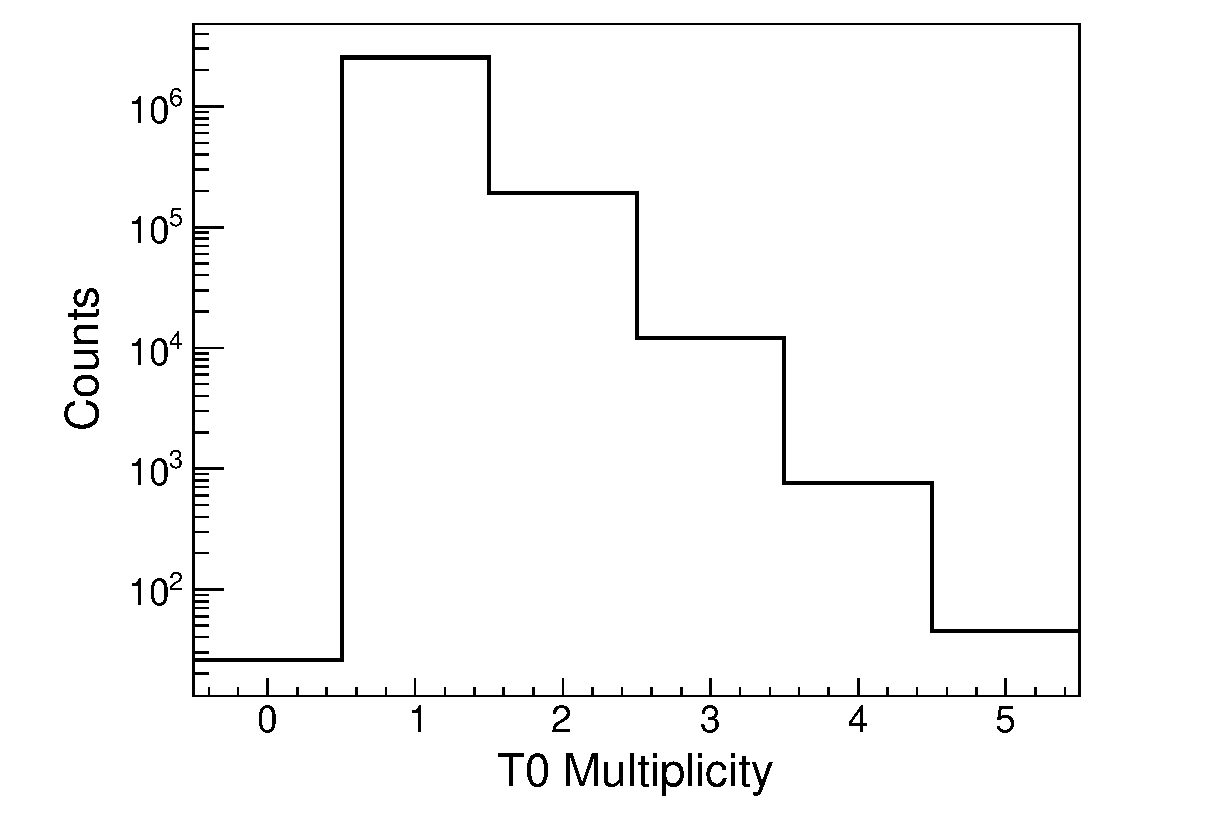
\includegraphics[width=5cm]{../pic/Run78/BL/nT0.eps}
    \end{minipage}

    \begin{minipage}{0.5\hsize}
      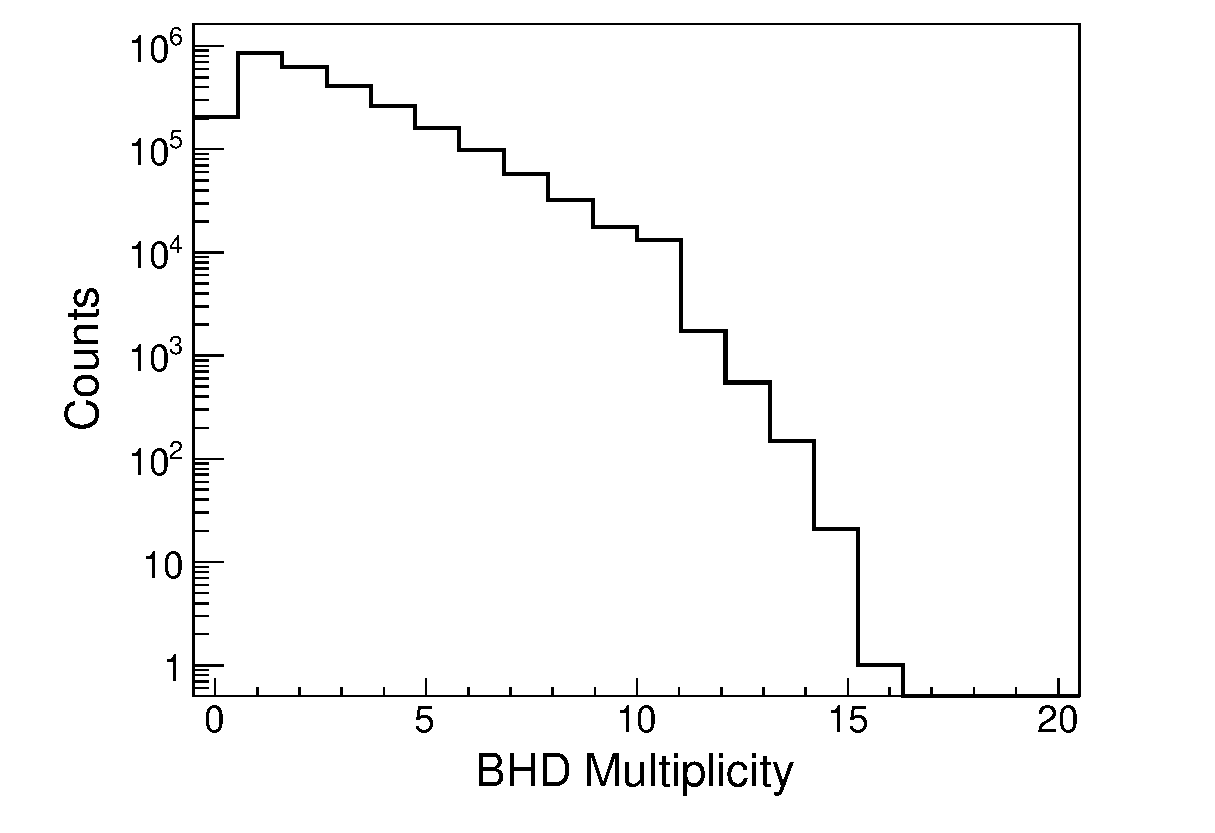
\includegraphics[width=5cm]{../pic/Run78/BL/nBHD.eps}
    \end{minipage}
  \end{tabular}
  \caption{
    These figures show the multiplicity of T0 and BHD counter.
  }
  \label{fig:nBHDT0}
\end{figure}

\begin{figure}
  \centering
  \includegraphics[width=7cm]{../pic/Run78/BL/BHDT0_TOF.eps}
  \caption{
    BHD-T0 time-of-flight with 7.7m flight length.
    The red hatched plot indicates an acceptable reigion as a kaon.
  }
  \label{fig:BHDT0_TOF}
\end{figure}


  
